%
% File acl2021.tex
%
%% Based on the style files for EMNLP 2020, which were
%% Based on the style files for ACL 2020, which were
%% Based on the style files for ACL 2018, NAACL 2018/19, which were
%% Based on the style files for ACL-2015, with some improvements
%%  taken from the NAACL-2016 style
%% Based on the style files for ACL-2014, which were, in turn,
%% based on ACL-2013, ACL-2012, ACL-2011, ACL-2010, ACL-IJCNLP-2009,
%% EACL-2009, IJCNLP-2008...
%% Based on the style files for EACL 2006 by 
%%e.agirre@ehu.es or Sergi.Balari@uab.es
%% and that of ACL 08 by Joakim Nivre and Noah Smith

\documentclass[11pt,a4paper]{article}
\usepackage[hyperref]{acl2021}
\usepackage{times}
\usepackage{latexsym}
\renewcommand{\UrlFont}{\ttfamily\small}

% This is not strictly necessary, and may be commented out,
% but it will improve the layout of the manuscript,
% and will typically save some space.
\usepackage{microtype}

\aclfinalcopy % Uncomment this line for the final submission
%\def\aclpaperid{***} %  Enter the acl Paper ID here

%\setlength\titlebox{5cm}
% You can expand the titlebox if you need extra space
% to show all the authors. Please do not make the titlebox
% smaller than 5cm (the original size); we will check this
% in the camera-ready version and ask you to change it back.

% Import additional packages
\usepackage{graphicx}
\usepackage{enumitem}
\usepackage{todonotes}
\usepackage{fixltx2e}

\usepackage{amsmath}
\usepackage{algorithm,algorithmic}


\newcommand\BibTeX{B\textsc{ib}\TeX}

\title{BERT-based Rumour Identification and Analysis for Twitter Posts}

\author{ Student ID: 1133751 \\
 COMP90042 Natural Language Processing \\
}

%\author{Matthias Bachfischer \\
% Student ID: 1133751 \\
% COMP90042 Natural Language Processing \\
 % \texttt{mbachfischen@unimelb.edu.au} 
 % }

\date{}

\begin{document}
\maketitle
\begin{abstract}
With the ease of access to information and its rapid dissemination across the internet, it has become increasingly difficult to differentiate rumour information from non-rumour information. In order to find ways to combat this issue, the COMP90042 Project 2021 put forward the task of developing a rumour detection system and analysing the nature of rumours that are being propagated on Twitter.
\newline
In this paper, we propose three systems using the Transformer architecture that leverage the textual content of conversations on Twitter to identify rumours. We further use these systems to analyze a dataset of 17,548 conversations related to COVID-19 in order to understand the nature of these rumours rumours. To evaluate the performance of our systems, we submitted our models to the COMP90042 CodaLab competition where we managed to achieve an F1-score of 0.837 with our best-performing system \textit{BERTweet}.
\end{abstract}

\section{Introduction}
With an increase in the adoption of social media as a news source, it has become easier for social media users to share false information with millions of users. This can lead to the spread of so-called fake news and rumours which may manipulate the opinion of a huge number of people.
Given the volume of rumours that are being generated on a day-to-day basis, there is a need for automated identification of rumours to facilitate in content moderation, as manual identification of rumours would involve a huge amount of manual labour.
\newline
Rumour detection is a challenging problem because of its dynamically evolving nature and the ambiguity that is associated with regard to what can be defined as a rumour and what not \citep{RN675}. As an example, a post shared on Twitter\footnote{Twitter Website \url{https://twitter.com}} may contain an incorrect claim, but was not actually shared with the intent to spread misinformation.
In contrast to that, another post may contain conspiracy theories and may have been shared in order to actively mislead, but might as well include some unrelated, but correct facts. This makes the task of automatically identifying  rumours challenging and justifies the use of elaborate methods. 

\section{Related Work}
Over the last years, the topic of rumour identification and analysis has attracted significant attention in Academia and has been subject to studies in shared tasks such as RumourEval 2017 \citep{RN690} and RumourEval 2019 \citep{RN691}.
Depending to the type of data that is being used, approaches for rumour identification can be divided into three major categories: \textit{message-based}, \textit{propagation-based} and \textit{stance-based}.
\newline
\textit{Message-based methods} focus on rumour detection based on the textual contents of the tweets, including the source tweet as well as all retweets and comments related to that tweet. The textual content of Twitter messages often has direct signals for misinformation which can be used for rumour detection. In \citet{RN676}, a RNN model is trained to automatically learn representations from tweets for rumour detection. Another approach was proposed in \citet{RN671} who proposed a GRU-based architecture to perform rumour detection at an very early stage of the propagation.
These methods are frequently extended to also leverage non-textual features such as user profile data for rumour and misinformation detection. In \citet{RN673}, a variety of both text and user features from users’ text response and their user profiles were extracted before feeding them through a CNN-based classifier for rumour identification while in \citet{RN481}, features such as word sentiment and tweets with support / denial terms are used for rumour detection.
\newline
\textit{Propagation-based methods} exploit tweet propagation information for rumour classification. Even though these approaches require large amounts of metadata, they have also been able to achieve highly competitive performance.
Recently a novel approach has been proposed by \citet{RN679} where an extended tree-structured recursive neural network (RvNN) is used to model information propagation. 
In \citet{RN672}, a novel architecture that uses Recurrent and Convolutional Neural Networks to classify propagation paths of events on Twitter was used and in \citet{RN669}, a tree transformer model was leveraged to incorporate user interactions into the propagation classification.
\newline
\textit{Stance-based methods} try to determine the rumour stance of a post with respect to the previous tweet and the source tweet. A system that leverages BERT for stance identification was published by \citet{RN665}. Another architecture built on a combination of a CNN and BERT architecture is presented in \citet{RN480}.

\section{Dataset}
The task of this project was to develop a rumour detection system and analyse the nature of rumours that are being propagated on Twitter.
The dataset for this task was published the COMP90042 teaching team and consists of set of source tweets and their replies (incl. corresponding metadata) that has been extracted from the Twitter API\footnote{Twitter API \url{https://developer.twitter.com/en/docs/twitter-api/enterprise/data-dictionary/native-enriched-objects/tweet}}.
The training set contains a total of 4641 events which have been labeled as either \textit{RUMOUR} or \textit{NON-RUMOUR}. In order to evaluate the performance of the system, an additional development set has been made available. A detailed breakdown of the class distribution is presented in Table \ref{tab:dataset_class_distribution}.
\begin{table}
\centering
\setlength\tabcolsep{2pt}
\begin{tabular}{lccc}
\hline
\textbf{Dataset}         & Rumour & Non-Rumour & Total \\ \hline
Training set    & 1583   & 3058       & 4641  \\
Development set & 187    & 393        & 580   \\
Test set        & -      & -          & 581   \\ \hline
\end{tabular}
\caption{Class distribution for rumour detection dataset}
\label{tab:dataset_class_distribution}
\end{table}
The training set is imbalanced and the majority of the tweets (approx. 66\%) belong to the non-rumour class, whereas the remaining data (approx. 34\%) belongs to the rumour class.

\section{Experimental Setup}
In section \ref{sec:task_1_rumour_detection}, we present the three rumour detection systems that were used in our research.
All three systems were implemented in Python and make use of the Transformers library \citep{RN682} which provides access to various Transformer-based architectures such as BERT, RoBERTa and DistilBERT. 
\newline
The experiments reported in this paper were performed on a VM instance within the Google Cloud Platform running Debian 10 with a Nvidia Tesla K80 GPU.


\section{Task 1 - Rumour Detection}
\label{sec:task_1_rumour_detection}
The goal of task 1 was to build a binary classifier that can reliably predict whether a given tweet represents a rumour or not.
\newline
To evaluate the performance of different models on the dataset, we have implemented three classification systems: A BERT-based implementation which we refer to as \textit{PureBERT}, as well as an extension of this architecture that combines the BERT model with tabular data and which we refer to as \textit{MultimodalBERT}.
\newline
In addition to that, a third model which is built on a pre-trained language model for English Tweets \citep{RN683} has been implemented. We refer to this model as \textit{BERTweet}.

\subsection{PureBERT}
\label{sec:purebert}
The \textit{PureBERT} system leverages the BERT language model that was initially published by \citet{RN688}. The model was pre-trained on the BooksCorpus \citep{RN689} and English Wikipedia and leverages the transformer architecture to provide contextualized representations for downstream tasks.
\newline
The \textit{PureBERT} model used in this assignment was implemented using Tensorflow \citep{RN681} and uses the textual content of the source tweets and as well as of their corresponding replies for rumour classification. 
\newline
\newline
\textbf{Pre-processing routine}
\newline
Prior to training the models on the given data, we have employed the following pre-processing procedure to clean the data and remove Twitter-specific tokens:
\begin{enumerate}[noitemsep]
%\itemsep0em 
    \item For every twitter event in the dataset, extract the source tweet text and corresponding replies and concatenate them 
    \item Remove URLs and user mentions from the tweet texts
    \item Convert tweet texts to lower-case
\end{enumerate}
For our experiments with \textit{PureBERT}, we have used a variety of pre-trained BERT models that have been made available on Tensorflow Hub\footnote{Tensorflow Hub \url{https://tfhub.dev/google/collections/transformer_encoders_text/1}}. This includes
\begin{itemize}[noitemsep,topsep=2pt,parsep=0pt,partopsep=0pt]
    \item \verb|bert-base-uncased|
    \item \verb|bert-large-uncased|
    \item \verb|talkheads_ggelu_bert_en_base|
\end{itemize}
The models \verb|bert-base-uncased| and \verb|bert-large-uncased| refer to the models that were published in the original BERT paper \citep{RN688}, while \verb|talkheads_ggelu_bert_en_base| refers to an improved BERT architecture which uses talking-heads attention and a gated linear unit with GELU activation (these changes were proposed by 
\citet{RN685} and \citet{RN686}).
\newline
To provide input to the \textit{PureBERT} model, we first tokenize the input tweets via the tokenizer. For each tokenized input text.  we construct the following:
\begin{itemize}[noitemsep,topsep=2pt,parsep=0pt,partopsep=0pt]
    \item \textbf{input ids:} a sequence of integers identifying each input token to its index number in the \textit{PureBERT} tokenizer vocabulary
    \item \textbf{attention mask:} a sequence of 1s and 0s, with 1s for all input tokens and 0s for all padding tokens
\end{itemize}
We subsequently fine-tune the pre-trained BERT models on the given input for $7$ epochs with AdamW optimizer \citep{RN687} using a learning rate of $3e^{-5}$.


\subsection{MultimodalBERT}
The \textit{MultimodalBERT} model is built using an experimental framework called Multimodal-Toolkit which has been made available on Github\footnote{Multimodal Transformers Repository \url{https://github.com/georgian-io/Multimodal-Toolkit}}. It allows to incorporate numerical and categorical features for downstream classification. 
\newline
The data used by the \textit{MultimodalBERT} system has been subject to the same pre-processing routine as described in section \ref{sec:purebert}. In addition to that, a variety of hand-crafted metadata features have been produced. 
\newline
\newline
\textbf{Metadata Features}
\newline
The context metadata used by \textit{MultimodalBERT} can be categorized into tweet-level and user-level features. This approach was inspired by \cite{RN668} and is based on the observation that rumours may have different properties from non-rumours (e.g. rumours may be more likely to include links with unverified information). The full set of features that have been extracted are described in Table \ref{tbl:handcrafted_features}.
\begin{table}
\centering
\begin{tabular}{l}
\hline 
\textbf{Tweet-level features} \\ \hline
Number of retweets \\
Number of favorites \\
Whether tweet has a question mark \\
Whether tweet contains URLs \\
Number of URLs embedded in tweet \\
Whether tweet has native media \\
\hline
\textbf{User-level features} \\ \hline
Number of posts user has posted \\
Number of public lists user belongs to \\
Number of followers \\
Number of followings \\
Whether user has a background image \\
Number of tweets user has liked so far \\
Whether user is verified\\
Whether geolocation is enabled \\
\hline
\end{tabular}
\caption{Description of metadata features}
\label{tbl:handcrafted_features} 
\end{table}
\begin{figure}[h]
\centering
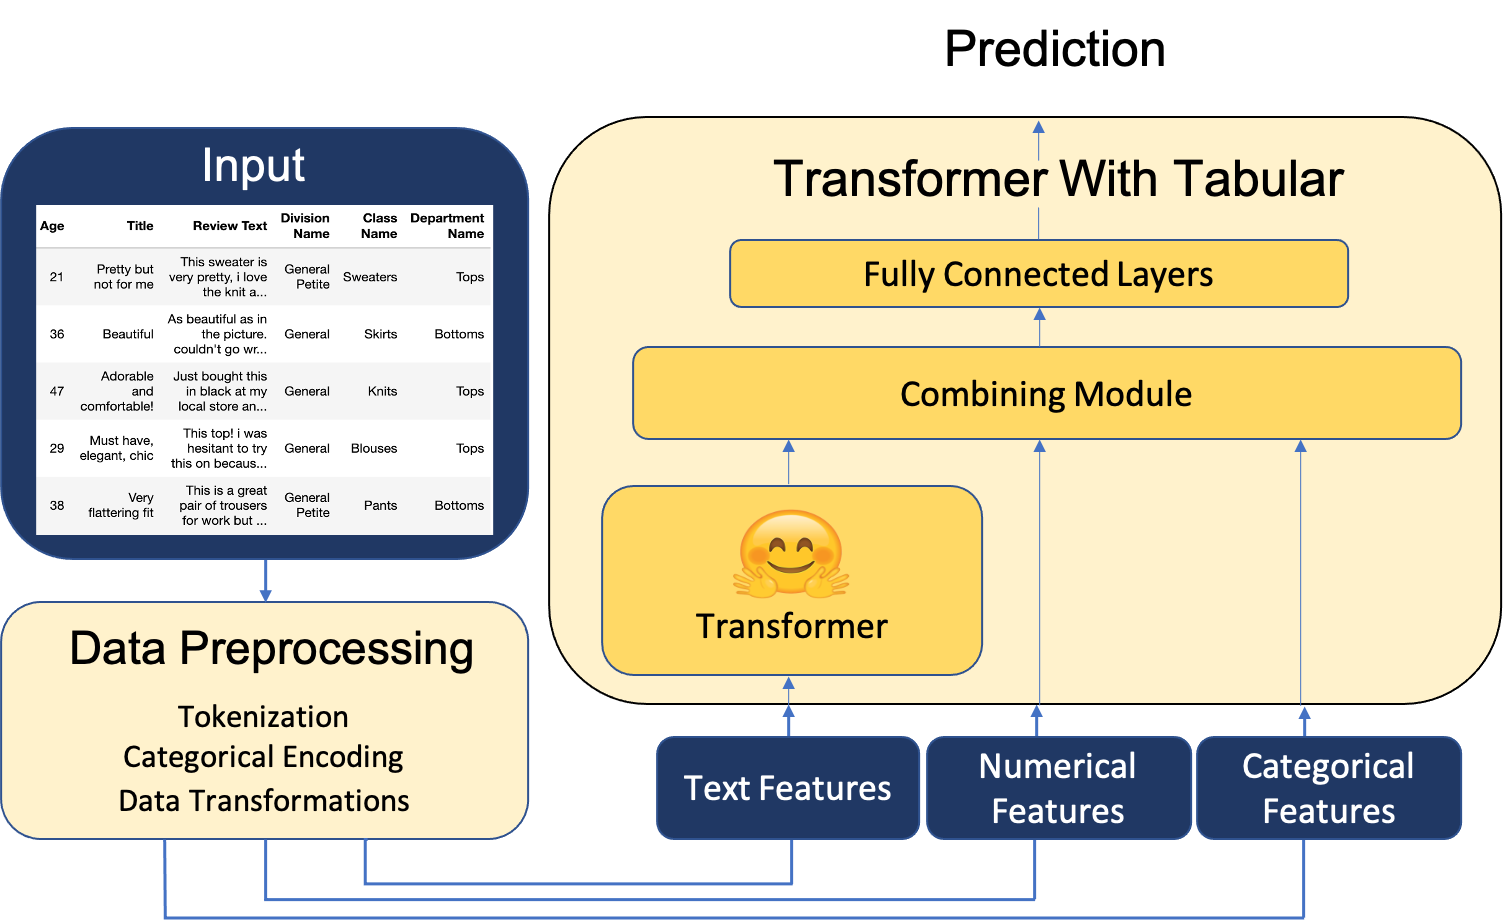
\includegraphics[width=0.45\textwidth]{images/multimodal_bert}
\caption{MultimodalBERT architecture}
\label{fig:multimodal_bert_architecture}
\end{figure}
\newline
Figure \ref{fig:multimodal_bert_architecture} gives an overview of the \textit{MultimodalBERT} architecture is given in Figure. We have performed various experiments in which we used a gated summation of the transformer outputs as well as the numerical and categorical features before the final classifier layer (a Multilayer Perceptron). Unfortunately we have not been able to achieve satisfactory performance on the task and have therefore discontinued the approach.

\subsection{BERTweet}
The \textit{BERTweet} model was published by \citet{RN683} and has been pre-trained on a corpus of 850M English Tweets. We put forward the hypothesis that tweets are fundamentally different from traditional text in terms of sequence length and the use of informal language. Hence, a language model pre-trained on a large corpus of tweets should achieve a better performance compared to a language model pre-trained on more formal language like Wikipedia.
\newline
We have implemented the \textit{BERTweet} model using the PyTorch framework \citep{RN684}. Since BERTweet comes with its own tokenizer \verb|BertweetTokenizer| that supports raw Twitter data, no pre-processing has been applied to the tweet texts at all.
To provide input to the \textit{BERTweet} model, we first tokenize the input tweets via the tokenizer. For each tokenized input text.  we construct the following:
\begin{itemize}[noitemsep,topsep=2pt,parsep=0pt,partopsep=0pt]
    \item \textbf{input ids:} a sequence of integers identifying each input token to its index number in the BERTweet tokenizer vocabulary
    \item \textbf{attention mask:} a sequence of 1s and 0s, with 1s for all input tokens and 0s for all padding tokens
\end{itemize}
We subsequently fine-tune the pre-trained BERTweet model on the given input for $7$ epochs with AdamW optimizer \citep{RN687} using a learning rate of $5e^{-5}$, and an epsilon value of $1e^{-8}$.

\subsection{Results}
The results of the proposed models in the COMP90042 CodaLab competition is shown in Table \ref{tbl:evaluation_scores}.
\begin{table}
\centering
\small
\setlength\tabcolsep{2pt}
\begin{tabular}{lccc}
\hline 
\textbf{Model / Features} & Precision & Recall & F1 Score \\ \hline
PureBert\textsubscript{base} & 0.843 & 0.745 & 0.791 \\ %v9
PureBert\textsubscript{large} & 0.813 & 0.829 & 0.821 \\ %v11
PureBert\textsubscript{talking heads} & 0.854 & 0.809 & 0.831 \\ %v16
BERTweet & 0.856 & 0.819 & 0.837 \\ %v18
MultimodalBert  & & not submitted \\
\hline
\end{tabular}
\caption{Evaluation scores}
\label{tbl:evaluation_scores}
\end{table}
From the table, it is evident that increasing the number of layers as well as the number of parameters enhances the performance of BERT (\textit{PureBert\textsubscript{base}} vs. \textit{PureBert\textsubscript{large})}. The performance of BERT with respect to the F1 score has further been improved by leveraging an updated BERT architecture (\textit{PureBert\textsubscript{talking heads}}). The model using the pre-trained \textit{BERTweet} model outperforms all other methods 
\newline
The above results support the hypothesis that that the language that is used in tweets is fundamentally different from regular natural language and hence a custom model fine-tuned exclusively on tweets is more suited for the classification of Twitter posts than a language model trained on regular English Language.

\section{Task 2 - Rumour Analysis}

Perform some analyses to understand the nature COVID-19 rumours and how they differ to their non- rumour counterparts...

\section{Conclusion}

\newpage
\bibliographystyle{acl_natbib}
\bibliography{acl2021}

%\appendix



\end{document}
